\subsection{Planejamento de trajetória}

O conhecimento de todas as regiões que podem ser recobertas pelo robô ajudam na
validação do posicionamento do robô. Porém, ainda é necessário descrever o
caminho a ser percorrido pelo efetuador no espaço de trabalho de maneira a
cumprir os requisitos de revestimento e o respectivo caminho percorrido no espaço de juntas.

A definição desse caminho é facilitada pelo conhecimento analítico da
superfície. A partir dessa descrição são definidos, sobre a pá, uma série
de faixas que segmenta a pá, que serão chamadas de
paralelos.

Os paralelos são espaçados de 3 em 3 milímetros para o cumprimento das exigência
de revestimento e são dispostos de forma a não possuirem intersecção entre si. A
união dos paralelos (considerando uma faixa de 3mm entre eles) inclui todos os
pontos da pá, garantindo seu completo recobrimento.

O deslocamento da ferramenta de revestimento  pelo caminho definido por dois
paralelos é feito por meridianos. Isto é, segmentos que
conectam extremidades dos paralelos e não tem função defininda no processo de
metalização. A vávula deve estar fechada e o revestimento interrompido
durante o tempo que o efetuador percorre todo o meridiano. A razão de existência
dele é meramente definir uma maneira de levar o efetuador de um paralelo a
outro.

\subsubsection{Modelagem da superfície}\label{modelagem}

Existem diversas abordagens matemáticas para descrição de superfícies como:
Parametrização Polinomial; Polinômios em três variáveis; Superfícies de
Bézier (\cite{farin2002curves}); Splines e NURBS (\textit{Non-uniform
rational B-spline}); Subdivisão de superfícies (\cite{peters2008subdivision}); Malhas
poligonais.

Todas essas formas de representar uma superfície, com excessão das malhas,
recaem em alguma instância em uma descrição polinomial. Dentre essas a única
descrição que ocorre de maneira implícita é por polinômios em três variáveis,
descrevendo uma variedade algébrica bidimensional, enquanto as demais são
parametrizações da superfície. 

Por simplicidade, fácil manipulação algébrica e implementação, a descrição
puramente polinomial (implícita) foi escolhida como abordagem inicial. De
maneira geral a superfície é descrita como o conjunto solução sobre os
números reais da equação polinomial ($f(x,y,z)=0$) de grau $N$, dito grau da
superfície, em $x$,$y$ e $z$:
\[\sum\limits_{i+j+k \leq N}^{} C_{i,j,k}x^iy^jz^k = 0\]

Os coeficientes $C_{i,j,k}$, então, são aqueles que descrevem da superfície.
Devido a restrição do grau do polinômio, o número de coeficientes é
$\binom{N+3}{3}$. Podendo ser vistos como coordenadas da superfície num espaço
projetivo de dimensão igual ao número de coeficiente,
$\mathbb{P}^{\binom{N+3}{3}}$, em outras palavras a superfície é invariante a
escalamento dos coeficientes.

Experimentalmente foi indentificado que um polinômio de quarto grau é suficiente
para aproximar toda uma região de interesse da pá, onde será feito o revestimento
para uma posição do robô, com erro submilimétrico. Nesse caso, o número de
coeficientes que devem ser identificados é $\binom{7}{3}$, ou seja, 35.

Com base no artigo de \cite{juttler2002least}, a conversão da descrição da
superfície de nuvem de pontos para uma descrição analítica foi feita utilizando
a informação da direção da normal à superfície em cada ponto, ou seja, a superfície analítica deve não apenas passar
próxima aos pontos da nuvem como deve também ter seu vetor normal similiar à
normal desses pontos.

Explorando o fato que polinômio são lineares em seus coeficientes, um sistema
superdeterminado, a ser resolvido por mínimo quadrados(\textit{curve fitting}
\cite{arlinghaus1994practical}) , foi contruído a partir do cálculo dos termos
do polinômio em cada ponto da nuvem (fazendo $f(x,y,z)=0$) e da avaliação da
normal em cada ponto, que deveria concordar com o gradiente do polinômio (ou
seja $\nabla f(x,y,z) = \overrightarrow{n}$, onde $\overrightarrow{n}$ é a
normal no ponto $(x,y,z)$ da nuvem), dessa forma o peso dado aos vetores normais
das amostras é igual ao peso das amostras.

%Elael Modelo Polinomial multivarial -> extrapolado para a pá inteira
% PREMISSAS!!


% 
% Splines
% Bézier Surface
% Runge's phenomenon
% Multivariate Polynomial fitting

\subsubsection{Cálculo dos paralelos}\label{paralelos}
% como subdividir em segmentos as regiões PREMISSAS!!
Na literatura, há diversas formas de dividir a superfície a ser revestida em
subregiões. Em \cite{from2010off}, por exemplo, um manipulador realiza a pintura
de uma superfície (\textit{spray gun}) cobrindo subregiões de um plano, projeção
%TODO nao entendi
 da superfície (figura~\ref{fig::pal}). Outra possibilidade é,
em funções
paramétricas, realizar uma trajetória semelhante à figura~\ref{fig::pal} no
espaço dos parâmetricos, cuja transformação (jacobiano) mapeará nos 'cortes' curvos da
superfície.

\begin{figure}[!ht]
	\centering	
	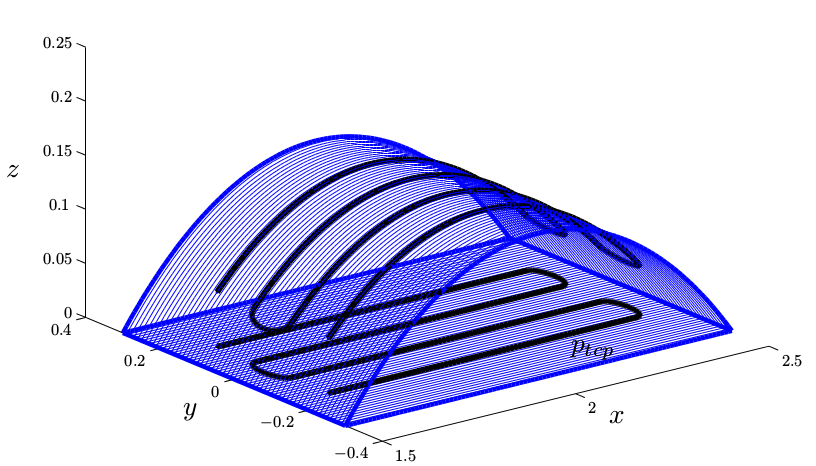
\includegraphics[width=\columnwidth]{method/figs/planejamento/pal.png}
	\caption{Subregiões de uma superfície.}
	\label{fig::pal}
\end{figure}



A superfície descrita na seção~\ref{modelagem} é uma equação implícita, na forma
$f(x,y,z)=0$. Neste caso, as trajetórias a serem percorridas pelo manipulador
podem ser obtidas através da interseção (cortes) entre planos uniformemente
espaçados e a superfície, o que gerará curvas ao seu longo. Uma
ideia semelhante e propícia devido à geometria do rotor, é gerar as curvas a partir da interseção
entre esferas e a superfície. As figuras~\ref{fig::interfrontal}
e~\ref{fig::interiso} mostram duas visões de duas interseções entre esferas e
a pá, onde as interseções estão representadas em vermelho, e as esferas em
azul claro. Os mesmos cortes podem ser observados entre esferas e o modelo
algébrico da pá, em figura~\ref{fig::intergeo}, na qual a pá está representada
em vermelho, as esferas estão em cinza claro, e as interseções são as curvas
sombreadas em cinza na pá.

A superfície descrita na seção~\ref{modelagem} é um subconjunto de uma
variedade algébrica de dimensão dois, representada na forma $f(x,y,z)=0$ como
uma imersão em $\mathbb{R}$, sendo assim uma superfície implícita onde
$f(x,y,z)$ é um polinômio nas três variáveis .
% Neste caso, trajetórias a serem percorridas pelo manipulador podem ser obtidas através da interseção (cortes)
% entre planos uniformemente espaçados e a superfície, o que gerará curvas ao
% longo da superfície. Uma ideia semelhante e propícia devido à geometria do
% rotor, é gerar as curvas a partir da interseção entre esferas e a superfície. 
As
figuras~\ref{fig::interfrontal} e~\ref{fig::interiso} mostram duas visões de
duas interseções entre esferas e a pá, onde as interseções estão representadas
em vermelho. Os mesmos cortes podem ser observados entre esferas e o modelo
algébrico da pá, em figura~\ref{fig::intergeo}.


\begin{figure}[!ht]
	\centering
	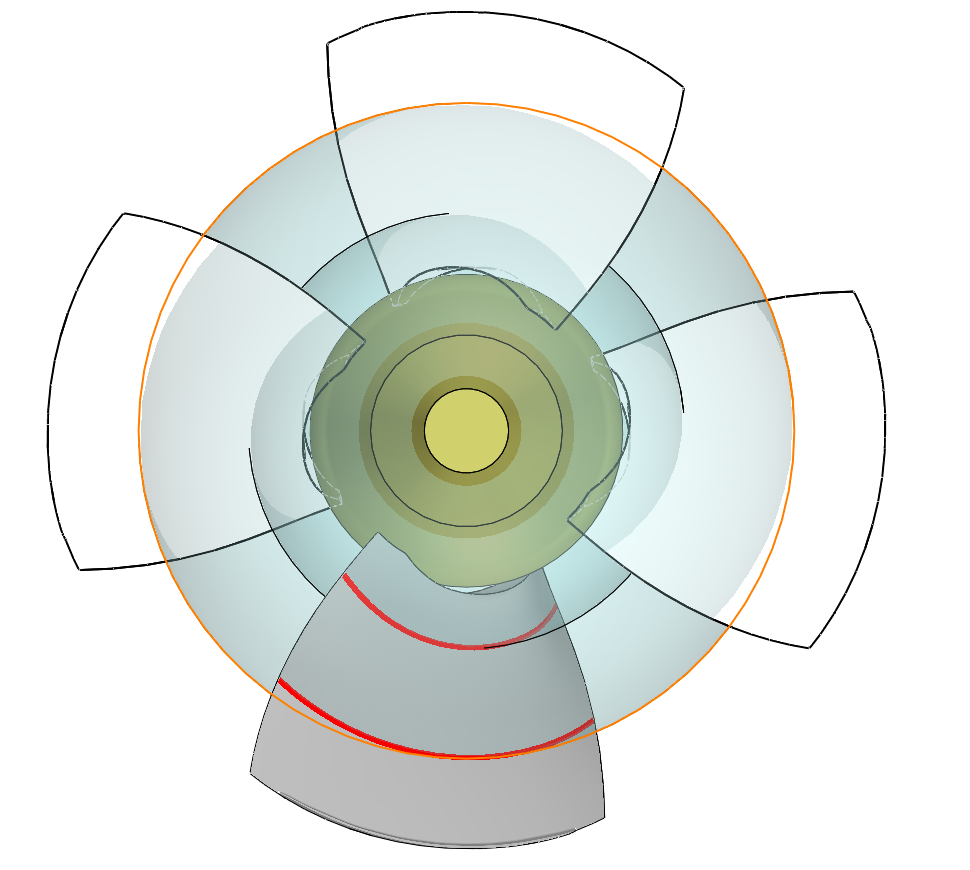
\includegraphics[width=.7\columnwidth]{method/figs/planejamento/intersecao_frontal.PNG}
	\caption{Interseção esfera-pá, vista frontal.}
	\label{fig::interfrontal}
\end{figure}

\begin{figure}[!ht]
	\centering
	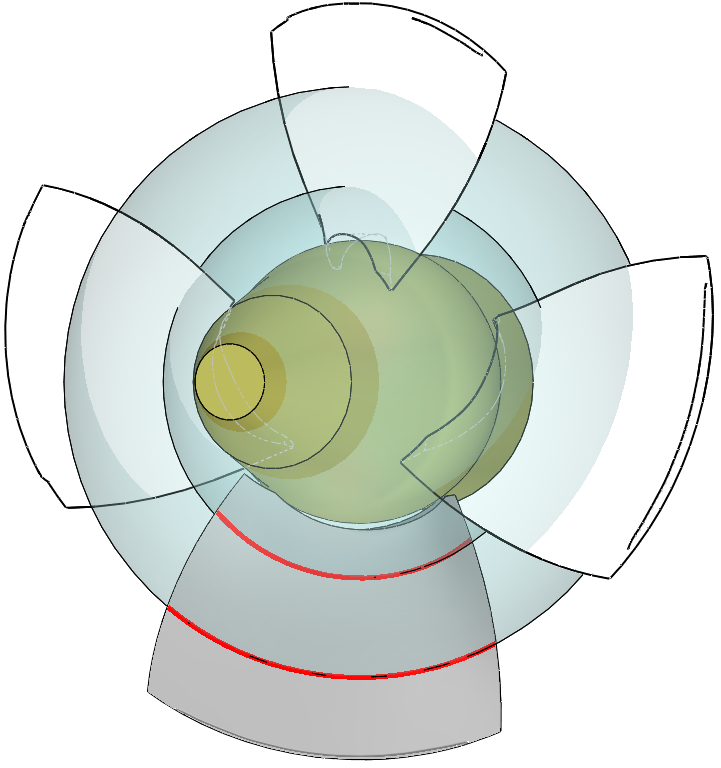
\includegraphics[width=.6\columnwidth]{method/figs/planejamento/intersecao_iso.PNG}
	\caption{Interseção esfera-pá, vista isométrica.}
	\label{fig::interiso}
\end{figure}

\begin{figure}[!ht]
	\centering
	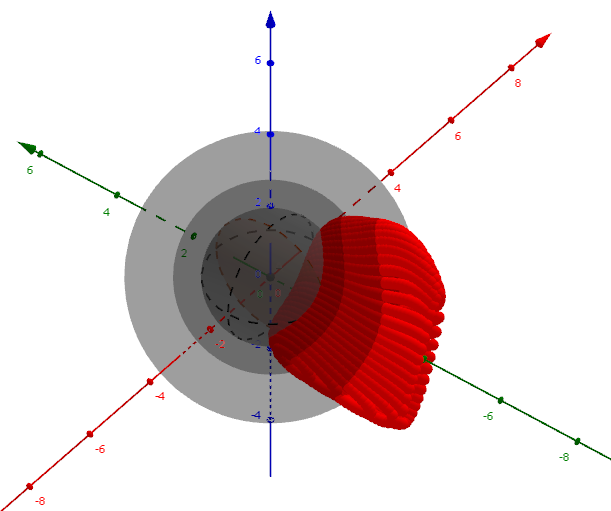
\includegraphics[width=\columnwidth]{method/figs/planejamento/intersecao_geogebra.png}
	\caption{Interseção esfera-modelo pá.}
	\label{fig::intergeo}
\end{figure}

A interseção de duas superfícies, a superfície da esfera
$g(x,y,z)=x^2+y^2+z^2-R^2=0$ e a superfície da pá $f(x,y,z)=0$, gera o caminho
que deve ser percorrido pelo robô. Porém, resolver algebricamente
$f(x,y,z)=g(x,y,z)$ é muito custoso, haveria a necessidade de
calcular as soluções para os ângulos das juntas do robô posteriormente, e ainda
realizar cáculos de restrição de borda da superfície, já que a função algébrica
encontrada para a pá é contínua e pode ter comportamento estranho fora da
região de interesse. Portanto, foi desenvolvido um método iterativo para a
computação da trajetória do robô de forma que, ao mesmo tempo que o caminho é
criado, os ângulos das juntas são computados, otimizando localmente a variação
dos ângulos das juntas, verificando restrição de ângulo de revestimento, e
bordas.

O método será explicado a partir de um exemplo genérico: suponha a superfície
algébrica da pá em vermelho, o rotor em preto, e a área que pode ser
revestida dada uma base do robô em amarelo, na figura~\ref{fig::vetores_out}.
Nesta etapa de revestimento (robô nesta posição de base), devem ser calculadas
as curvas (trajetórias). É selecionado o ponto central da núvem de
pontos revestidos (em amarelo), e é calculado o ponto mais próximo à superfície,
representado como ponto $B$ da figura~\ref{fig::vetores_out2}.
$\vec{AB}$ é o vetor normal à esfera, igual a $\vec{OB}$ (origem ao ponto B), e $\vec{BC}$ é o vetor normal à superfície
algébrica da pá, calculado como $\nabla{f} = \vec{f_x,f_y,f_z}$. O vetor
tangente $\vec{BD}$, figura~\ref{fig::vetores_in}, pode ser calculado como
produto vetorial entre o vetor normal à superfície da pá com o vetor normal à
esfera, no ponto B: $\vec{BD} = \vec{BC} \times \vec{AB} = \vec{OB} \times
\nabla{f}$. A integral do vetor tangente irá fornecer a trajetória (região
cinza sombreada, ou em vermelho, como na figura~\ref{fig::interiso}), logo o
caminho (ou trajetória) é calculado por:
$$c = \int \vec{OB} \times \nabla{f} dt.$$ 

Em integrações numéricas, deve-se garantir que o novo ponto de cada iteração
pertença à superfície, logo $B' = B + \int_0^t \vec{OB} \times \nabla{f} dt$, onde $t$ é o passo de integração, não é
suficiente, pois deve-se reprojetar o novo ponto $B'$ na superfície da pá. Isso
é feito por uma otimização, enunciada da seguinte forma:
$$min \left \| B-B' \right \|^2$$
$$s.t. f(B')=0$$
E assim garante-se que o novo ponto $B'$ pertence à superfície da pá.

Em cada passo da integração numérica, deve-se computar a solução dos ângulos das
juntas (cinemática inversa) para o revestimento. Caso não haja solução, ou o
ângulo entre avanço do efetuador e normal da pá seja maior que $30^o$, a trajetória está
concluída e a integração é interrompida. Calculam-se os valores dos ângulos das
juntas em cada passo por uma otimização, enunciada da seguinte forma:
$$min -\nabla{f}\cdot x_T$$
$$s.t. \left \| p_T-B \right \|^2=0$$
Onde $x_T$ são as três primeiras linhas da primeira coluna da transformação
homogênea $T_{bB}$ ($b$ é a base do manipulador), pois o vetor de avanço do
efetuador do manipulador é $x=(1,0,0)$, logo a primeira coluna. E $p_T$ são as
três primeiras linhas da quarta coluna da transformação
homogênea $T_{bB'}$, representando a posição do efetuador.

\begin{figure}[!ht]
	\centering
	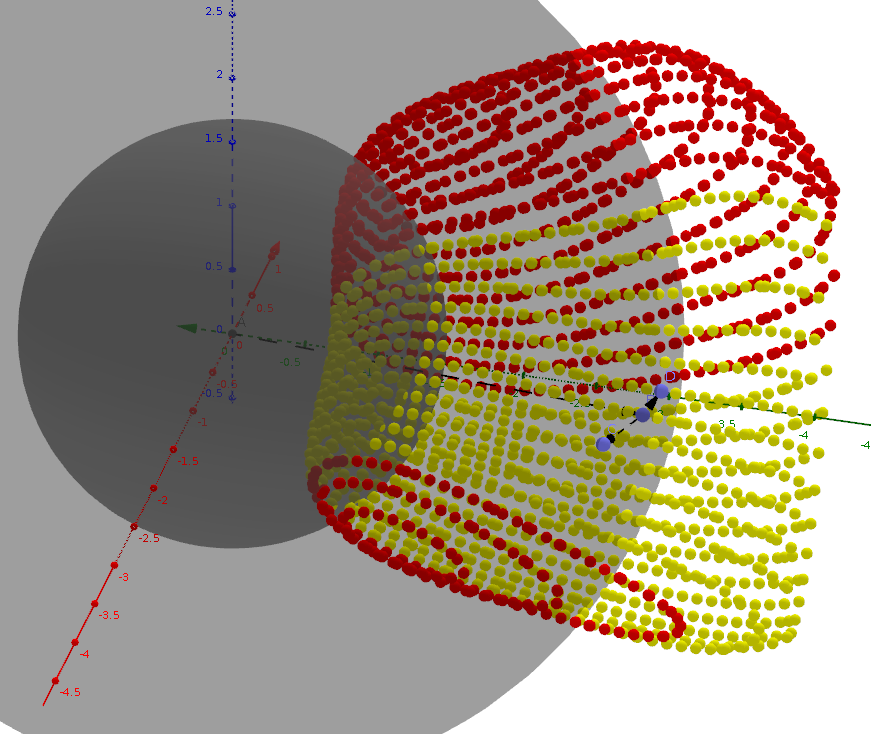
\includegraphics[width=\columnwidth]{method/figs/planejamento/vetores_out.png}
	\caption{Vetores de interesse na interseção esfera-pá.}
	\label{fig::vetores_out}
\end{figure}

\begin{figure}[!ht]
	\centering
	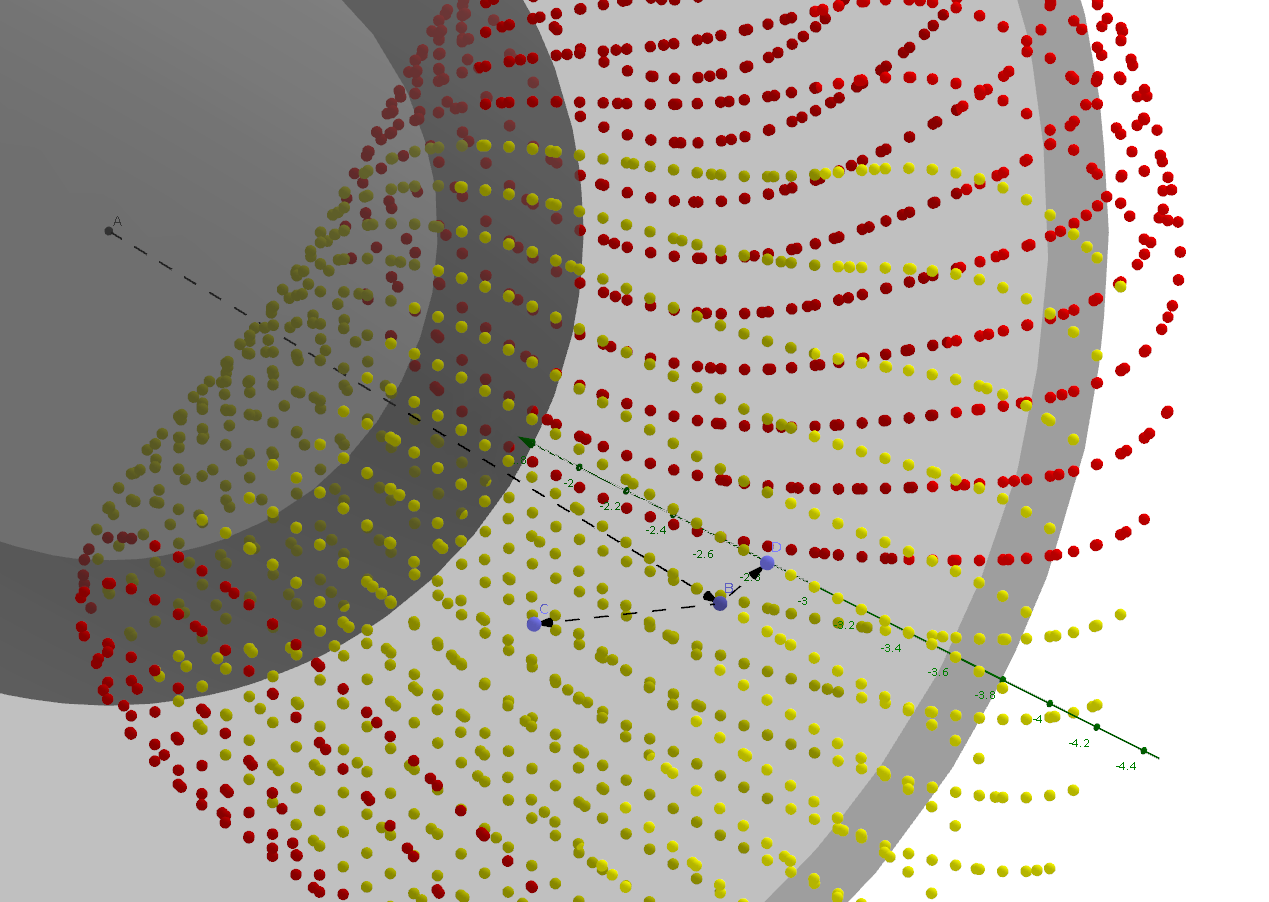
\includegraphics[width=\columnwidth]{method/figs/planejamento/vetores_out2.png}
	\caption{Vetores de interesse na interseção esfera-pá.}
	\label{fig::vetores_out2}
\end{figure}

\begin{figure}[!ht]
	\centering
	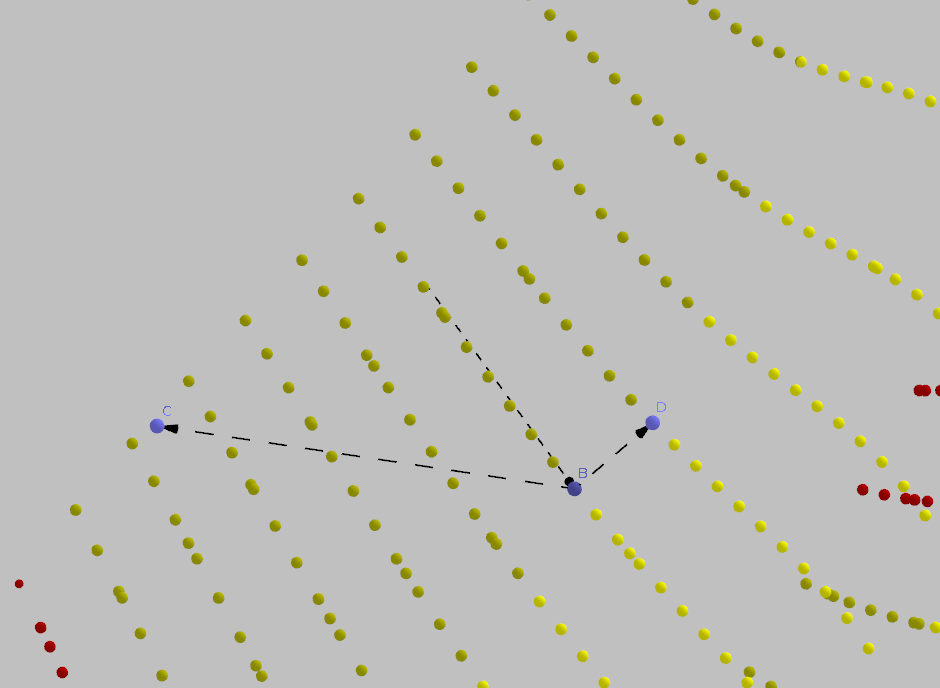
\includegraphics[width=\columnwidth]{method/figs/planejamento/vetores_in.png}
	\caption{Vetores de interesse na interseção esfera-pá.}
	\label{fig::vetores_in}
\end{figure}

A figura~\ref{fig::path_openrave} mostra duas curvas computadas pelo algoritmo
descrito acima. Os caminhos tem espaçamento exagerado, maior que 3 mm, para
facilitar a visualização. A transição entre os paralelos, no entanto, é
executada por outro algoritmo, que calcula os meridianos do planejamento de
trajetória.

\begin{figure}[!ht]
	\centering
	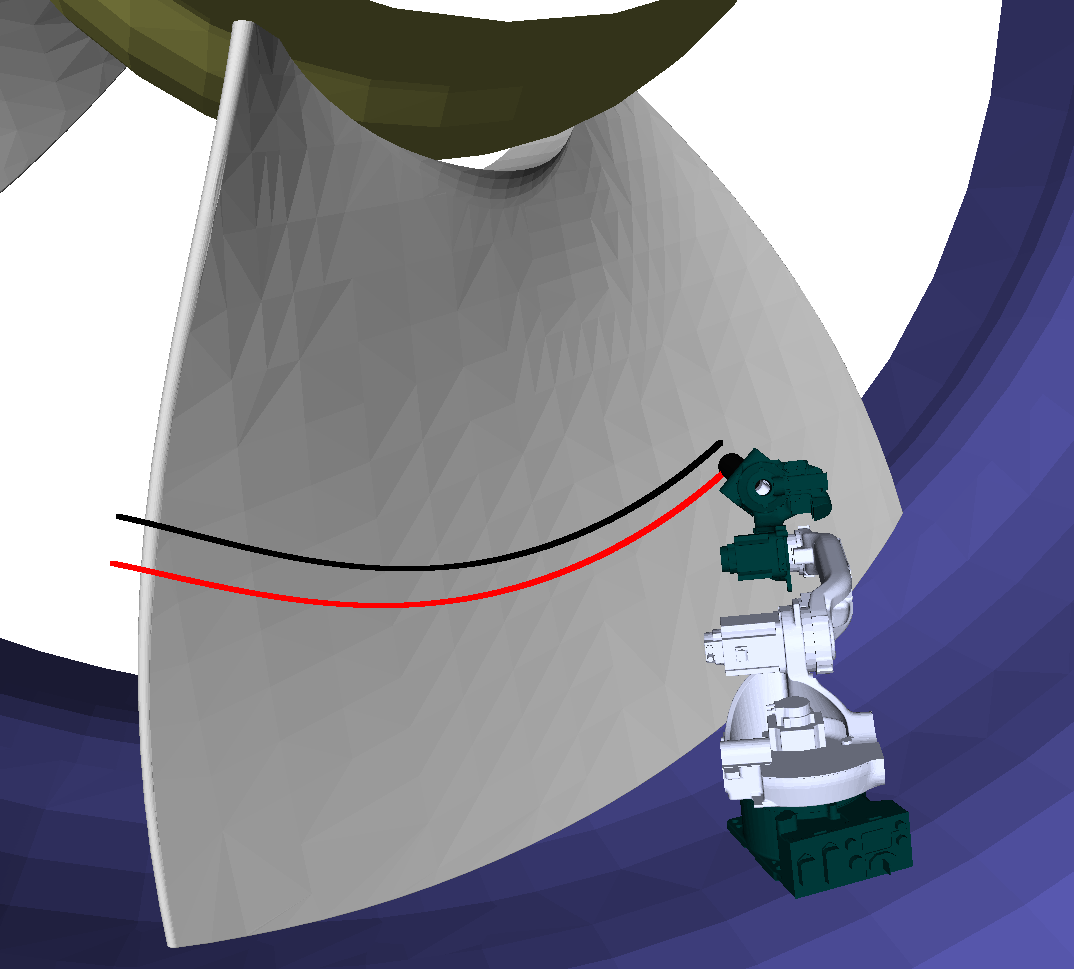
\includegraphics[width=\columnwidth]{method/figs/planejamento/path_openrave.png}
	\caption{Simulação de trajetória no Openrave.}
	\label{fig::path_openrave}
\end{figure}

\subsubsection{Cálculo dos meridianos}
Os paralelos, ou caminhos ``horizontais'', são computados pelo algoritmo
descrito na subseção~\ref{paralelos}. Entretanto, o algoritmo não descreve as
transições entre linhas horizontais, como se o manipulador ``pulasse''
de um paralelo a outro, o que não pode acontecer, já que o caminho deve ser
contínuo. Dessa forma, há a necessidade de computação das curvas de transição,
os caminhos ``verticais'', ou meridianos da superfície da pá.

Ao fim da execução do cálculo de um paralelo (por exemplo, ao fim do
cálculo da curva em vermelho da figura~\ref{fig::interiso}), o
efetuador estará apontando para o último ponto com solução viável neste
paralelo, dentro das restrições de ângulo de revestimento, no lado esquerdo ou direito. A partir
deste ponto extremo (borda), o manipulador deverá ``descer'' ou ``subir'' pelo
meridiano, até encontrar outro paralelo, isto é, encontrar outra curva que
satisfaça $f(x,y,z)=g(x,y,z)$.

O método será explicado a partir de um exemplo genérico: suponha que o efetuador
do manipulador se encontra como na figura~\ref{fig::path_openrave} (borda
direita), isto é, na extremidade direita de um paralelo $c_1$. Caminhar em um
meridiano significa integrar o vetor tangente perpendicular ao encontrado por $\vec{BD} = \vec{OB} \times
\nabla{f}$, logo o caminho pelo meridiano pode ser calculado
como:
$$m_{12} = \int (\vec{OB} \times \nabla{f})\times \nabla{f} dt$$
o que irá gerar um caminho de descida pelo meridiano. Em cada passo de
integração numérica, o novo ponto $B' = B + \int_0^t (\vec{OB} \times
\nabla{f})\times \nabla{f} dt$ deve ser projetado na superfície, como em
na subseção~\ref{paralelos}, pela otimização:
$$min \left \| B-B' \right \|^2$$
$$s.t. f(B')=0$$
Além disso, em cada passo deverá ser verificado se o caminho já alcançou o
próximo paralelo $c_2$, isto é, se o ponto pertence à esfera de raio
$R_2=R_1+0.003$ (em milímetros). Observe que se o o caminho passar do próximo
paralelo, o caminho deve ser feito no sentido contrário com passo menor, isto é:
$$m_{21} = \int -(\vec{OB} \times \nabla{f})\times \nabla{f} dt$$

Na figura~\ref{fig::meridianos}, os meridianos estão representados em verde.

\begin{figure}[!ht]
	\centering
	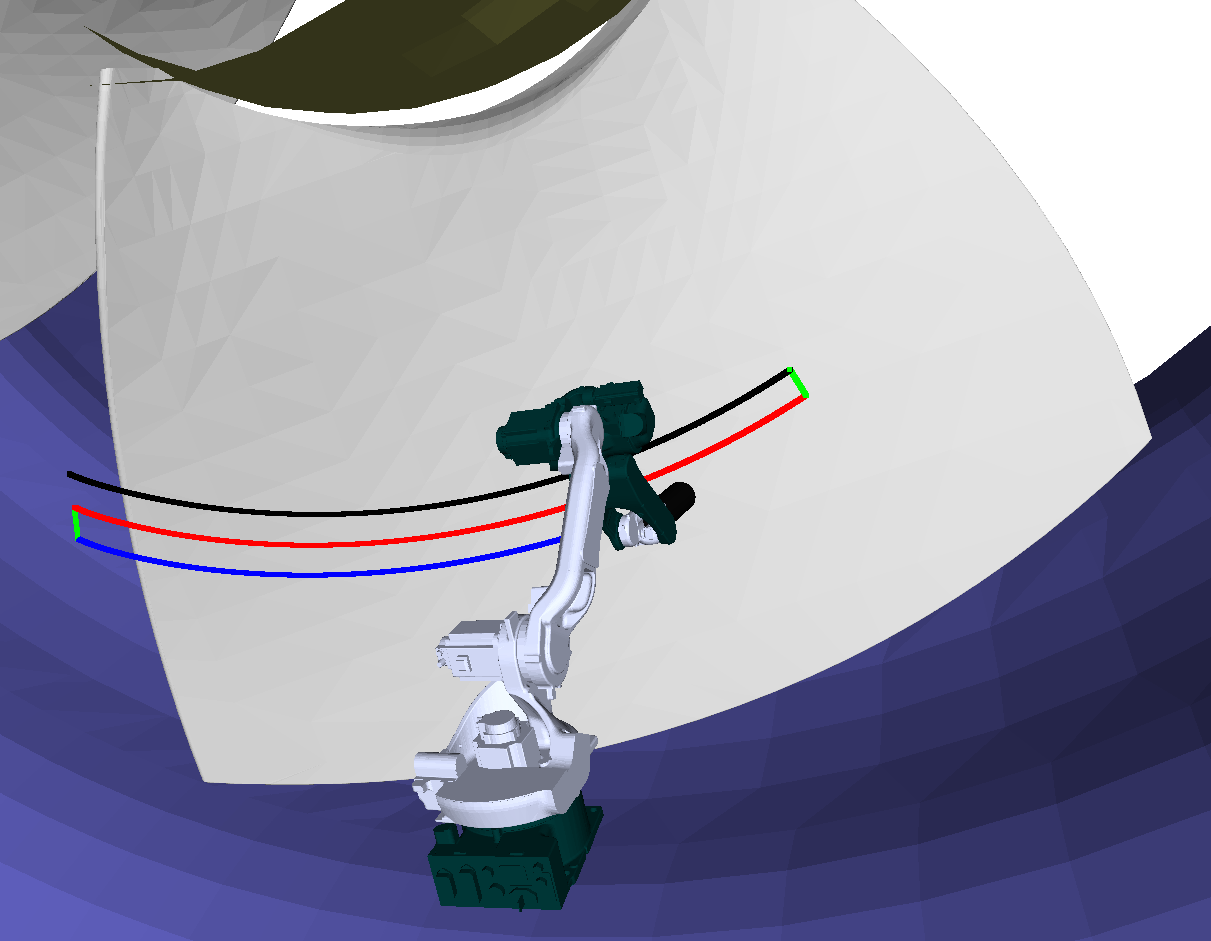
\includegraphics[width=0.7\columnwidth]{method/figs/planejamento/meridianos.png}
	\caption{Meridianos da pá.}
	\label{fig::meridianos}
\end{figure}

\subsection{Conclusão}

No âmbito do controle e planejamento de trajetória, o método desenvolvido já se
mostrou capaz de analisar a superfície da pá, segmenta-la em regiões e definir
caminhos para serem percorridos, tanto pelo efetuador (no espaço de trabalho)
quanto pelas juntas (no espaço de juntas).

Porém, validações da precisão do resultado e análise de colisão devem ser mais
exploradas. Também devem ser julgadas pequenas modificações do método como
aplicação de minímos quadrados móveis na definição da superfície, técnica 
que possibilitaria um maior controle do erro localmente.
